% =============================================================================
% Part 1: Abstract + Introduction
% (Abstract carries no citations. Contributions list appears at the END of the
%  Introduction, after the problem and the approach.)
% =============================================================================

\begin{abstract}
This work is relevant to researchers in continual learning, memory-augmented transformers, and biologically-inspired machine learning. We implement and empirically evaluate a biologically-faithful memory consolidation architecture for Large Language Models, drawing on the synaptic tagging-and-capture hypothesis, the Complementary Learning Systems framework, and hippocampal--neocortical replay during sleep. Our system, SLEEP, augments pretrained transformers with five interacting components: prediction-error tagging, direct-write key-value (KV) memory, protein-resource-allocation prioritization, generative replay, and LoRA-based consolidation under explicit safety constraints. The paper proceeds in two movements. The first is a diagnosis: across 200 single-exposure synthetic facts on four models spanning three families (Qwen2.5-7B and 1.5B, Llama-3.1-8B, Mistral-7B), five seeds each, the architecture as originally specified produces recognition without recall---memories that bias multiple-choice judgement but never surface in free-form generation, a floor of $\mathrm{DRA} \approx 0.006$ against in-context ceilings up to $0.99$---while its internal surprise-based validation falsely confirms $93$--$100\%$ of consolidations and a retrieval-aware warm-up repair fails in sixteen runs. The second movement locates and removes the causes. Guided by the knowledge-editing literature, we show the consolidation failure decomposes into three stacked errors: the adapter was in the wrong substrate (attention projections in the top third of layers, chosen by biological analogy, rather than the mid-stack MLPs where causal tracing places factual associations), it was trained on single wordings (producing memorization without extraction), and the safety machinery's hard clip erased what training wrote. Correcting all three---mid-stack MLP placement, paraphrase-diverse replay, distillation from an in-context teacher, and a moderate clip---raises single-cycle recall from the $0.006$ floor to $0.75$ on Mistral-7B (five seeds) with background damage near the acceptability bar, and to $17$--$125\times$ the floor on every model tested. In the multi-cycle regime the machinery was designed for, the repaired system beats naive LoRA on cumulative recall on all four models on both seeds ($3\times$ on Qwen2.5-7B), beats a matched EWC-only baseline ($0.174$ vs.\ $0.056$), and prevents the catastrophic damage blow-up that destroys the unconstrained baseline at 1.5B scale ($\mathrm{BCP}$ $2.4$ vs.\ $24.5$). All validation-phase gates and predictions were pre-registered before the experiments ran. The recognition--recall dissociation, the proxy-validation failure, and the horizon-and-seed instability of unconstrained baselines stand as diagnostic contributions; the localisation repair converts them from a negative result into a working, baseline-controlled system with named residual gaps.
\end{abstract}

\section{Introduction}
\label{sec:intro}

\begin{figure}[t]
\centering
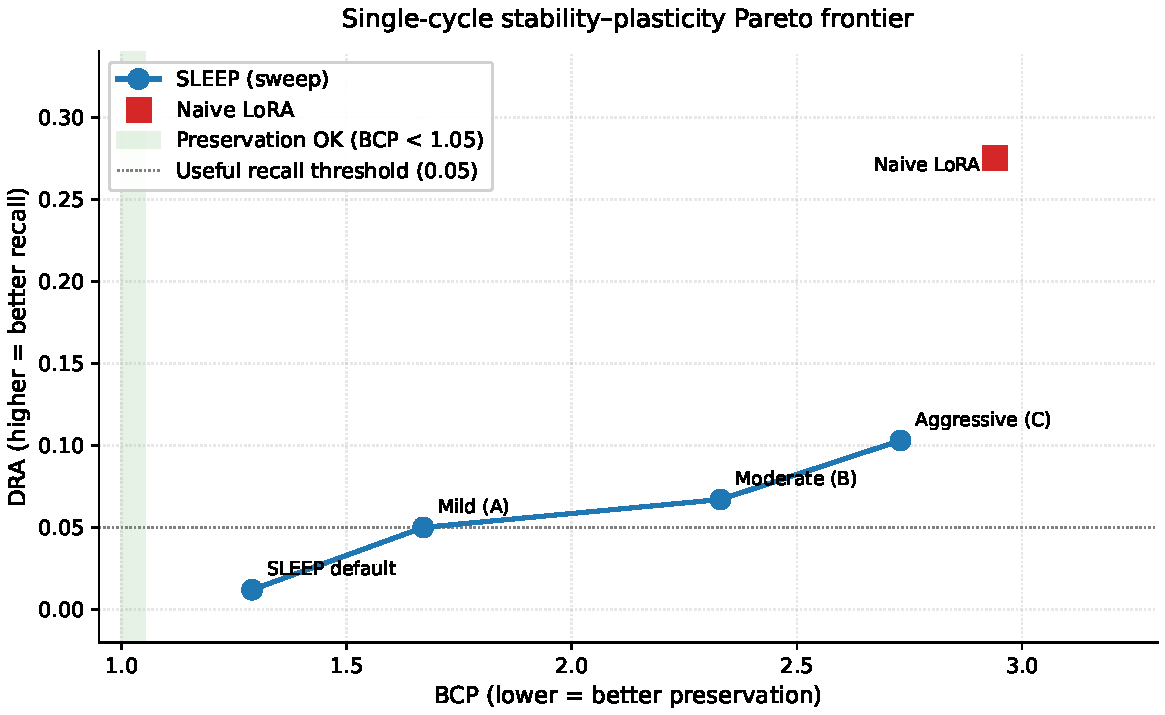
\includegraphics[width=0.78\textwidth]{figures/figure_pareto_frontier.pdf}
\caption{Single-cycle stability--plasticity Pareto frontier of the \emph{original} architecture (attention-top placement, single-wording replay). SLEEP configurations sweep from default (most conservative) to aggressive; naive LoRA marks the unconstrained extreme. The green band shows the preservation-acceptable region ($\mathrm{BCP} < 1.05$); the dotted line shows a useful-recall threshold ($\mathrm{DRA} > 0.05$). No setting on this frontier reaches the upper-left intersection---and Section~\ref{sec:results_localisation} shows why: the frontier itself is an artefact of consolidating into the wrong substrate. The localisation-corrected pipeline of Section~\ref{sec:results_pipeline_v2} reaches $\mathrm{DRA}=0.19$ at $\mathrm{BCP}=0.88$ on this model (five seeds), off this curve's scale.}
\label{fig:pareto}
\end{figure}

Large language models exhibit a form of architectural anterograde amnesia: pretrained weights are fixed at deployment, and any new information acquired during inference exists only within the context window, vanishing once the conversation ends. Retrieval-augmented generation (RAG) treats this as plumbing---append a database lookup to every query---rather than as a representational gap to close \citep{lewis2020retrieval}.

Biological memory faces an analogous problem and solves it through a structured pipeline: surprising experiences are flagged at the synapse by prediction-error-driven tags, those tags compete for a limited pool of plasticity-related proteins (PRPs), and the resulting episodic traces are gradually transferred from hippocampus to neocortex through replay during sleep. We review this literature in Section~\ref{sec:related} and Section~\ref{sec:background}; here we note only that the biological result is continuous, selective, single-exposure learning that does not catastrophically overwrite existing knowledge.

We propose SLEEP, a system that implements all five of these mechanisms---tagging, key-value (KV) memory, protein-resource allocation, sleep replay, and dual-weight consolidation---and evaluate each component in isolation across four models from three families. Following a pre-registered formalization in which 36 design questions were resolved before any code was written, we instrument every stage of the pipeline and identify exactly where information is preserved, transformed, or lost. This paper tells the story in the order the evidence forced it on us, in two movements.

\textbf{The first movement is a diagnosis.} The encoding components work: direct-write KV memory injection produces a clear recognition signal on multiple-choice evaluation. The consolidation components, as originally specified, do not: no configuration achieves a Delayed Recall Accuracy (DRA) above $0.05$ while holding Base Capability Preservation (BCP) below $1.05$, and the recall floor sits at $\mathrm{DRA} \approx 0.006$ on every one of four models across three families, five seeds each---from models that follow the same facts in context at up to $0.99$. The failure survives a principled repair attempt (a retrieval-aware warm-up; sixteen runs, no movement), the system's internal validation certifies consolidations at a $93$--$100\%$ false-confirmation rate everywhere, and long-horizon comparisons of the unconstrained baseline prove unstable in both horizon and seed.

\textbf{The second movement locates the causes and removes them.} The knowledge-editing literature places factual associations not where biological analogy placed our adapter (attention projections, top third of layers) but in mid-stack MLP modules. Guided by this, a five-arm isolation experiment shows the consolidation failure decomposes into three stacked causes: wrong substrate, single-wording training (which produces string memorization rather than extractable knowledge), and safety machinery whose hard clip erased the write. Correcting all three yields a repaired pipeline---mid-stack MLP placement, paraphrase-diverse replay, distillation from an in-context teacher, moderate clipping---that we then validate under pre-registered gates across the full matrix: five seeds per model single-cycle, ten-cycle continual learning against naive LoRA on all four models, and a matched EWC-only baseline. Single-cycle recall reaches $0.750 \pm 0.033$ on Mistral-7B---125 times the old floor---and exceeds it by at least $17\times$ everywhere. In the multi-cycle design regime the repaired system beats naive LoRA on cumulative recall on all four models on both seeds, beats EWC-only three-fold on the anchor model, and prevents the damage catastrophe that seed-randomly destroys the unconstrained baseline at small scale.

These findings yield the following contributions.

\paragraph{Contributions:}
\begin{enumerate}[label=(C\arabic*),itemsep=0.15em,topsep=0.2em,leftmargin=*]
    \item LoRA fast weights cannot encode at single exposure: $\alpha_{\mathrm{fast}} = 10^{-4}$ falls below the bfloat16 precision floor, and float32 testing shows the default magnitude is separately under-scaled at 7B.
    \item Direct-write KV memory injection produces recognition but not generative recall---a transformer analogue of the cognitive recognition--recall dissociation. The recall floor replicates at $\mathrm{DRA} \approx 0.006$--$0.007$ on four models across three families, five seeds each, while the same models follow in-context facts at up to $0.99$; a retrieval-aware warm-up moves recognition but never recall in sixteen runs.
    \item Internal validation passes while external recall fails: across all four models, $93$--$100\%$ of candidates that pass surprise-reduction fail a direct recall gate---a self-grading discrepancy not unique to SLEEP.
    \item Fixed-horizon, single-run comparisons of \emph{unconstrained} continual-learning baselines are unreliable: the damage trajectory of naive fine-tuning varies by up to three orders of magnitude across seeds of identical configurations, flipping fixed-horizon orderings seed to seed.
    \item The consolidation failure is causally decomposed into three stacked errors---substrate (attention-top vs.\ mid-stack MLP), surface diversity (single wording vs.\ paraphrases), and safety clipping---each isolated experimentally. Placement alone halves background damage in 8 of 8 comparisons; paraphrase diversity trades cloze accuracy for free-form recall (memorization $\to$ extraction); the designed clip nullifies the recipe ($0.007$) that a moderate clip preserves ($0.21 \pm 0.02$).
    \item The repaired pipeline generalises across families and scales under pre-registered gates: single-cycle trained-subset DRA of $0.750 \pm 0.033$ (Mistral-7B), $0.512 \pm 0.048$ (Llama-3.1-8B), $0.189 \pm 0.031$ (Qwen2.5-7B), and $0.105 \pm 0.020$ (Qwen2.5-1.5B), five seeds each---$17$--$125\times$ the original floor, strongest off the development model.
    \item In the ten-cycle regime the machinery was designed for, the repaired system beats naive LoRA on cumulative recall on 4 of 4 models (both seeds; $3\times$ on Qwen2.5-7B) and beats a matched EWC-only baseline ($0.174$ vs.\ $0.056$): regularization prevents forgetting but does not create extraction. Right-sized safety machinery is load-bearing at small scale, holding BCP near $2.4$ where naive LoRA blows up to $24.5$, and reduces across-seed variance by an order of magnitude.
\end{enumerate}

The claim structure is deliberately scoped. The diagnostic findings (C1--C4) replicate across every model we can test at this scale. The repair (C5--C7) is validated across three families and two scales with pre-registered gates, with one family flagged: Llama-3.1-8B gains recall like the others but no tested clip setting yet holds its background damage inside our acceptability bar, so we report it as \emph{not yet tuned} rather than solved. We release the implementation, formalization, pre-registrations, experimental logs, and all 35 validation-phase runs.
